\documentclass[10pt, a4paper]{article}

\usepackage[paper=a4paper, left=1.5cm, right=1.5cm, bottom=1.5cm, top=1.5cm]{geometry}
\usepackage[utf8]{inputenc}
\usepackage[spanish]{babel}
\usepackage{graphicx}
\usepackage{multicol}
\usepackage[usenames,dvipsnames]{color}
\usepackage{amsmath}
\usepackage{verbatim}
\usepackage{footnote}
\usepackage{float}
\usepackage{amsfonts}
\usepackage{hyperref}
\usepackage{framed}
\usepackage{pdflscape}

\usepackage{pdfpages}


\newcommand{\escaladefault}{0.85}

\begin{document}


\section{Introducción}

\subsection{Work Breakdown Structure} 

Incluimos un WBS híbrido de procesos y productos, para ilustrar los subcomponentes del proyecto.

\begin{figure}[H]
\centering
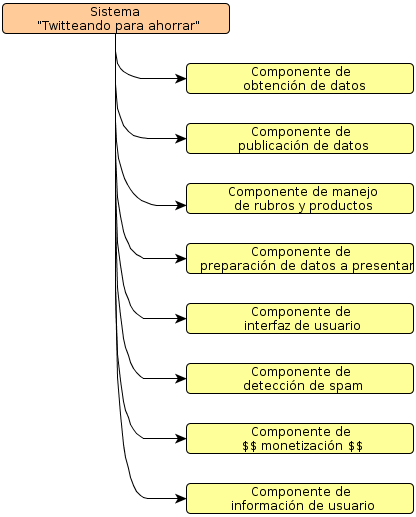
\includegraphics[scale=\escaladefault]{graficos/wbs/primera_capa.png}
\caption{Vista general del WBS: componentes del proyecto}
\end{figure}


\begin{figure}[H]
\centering
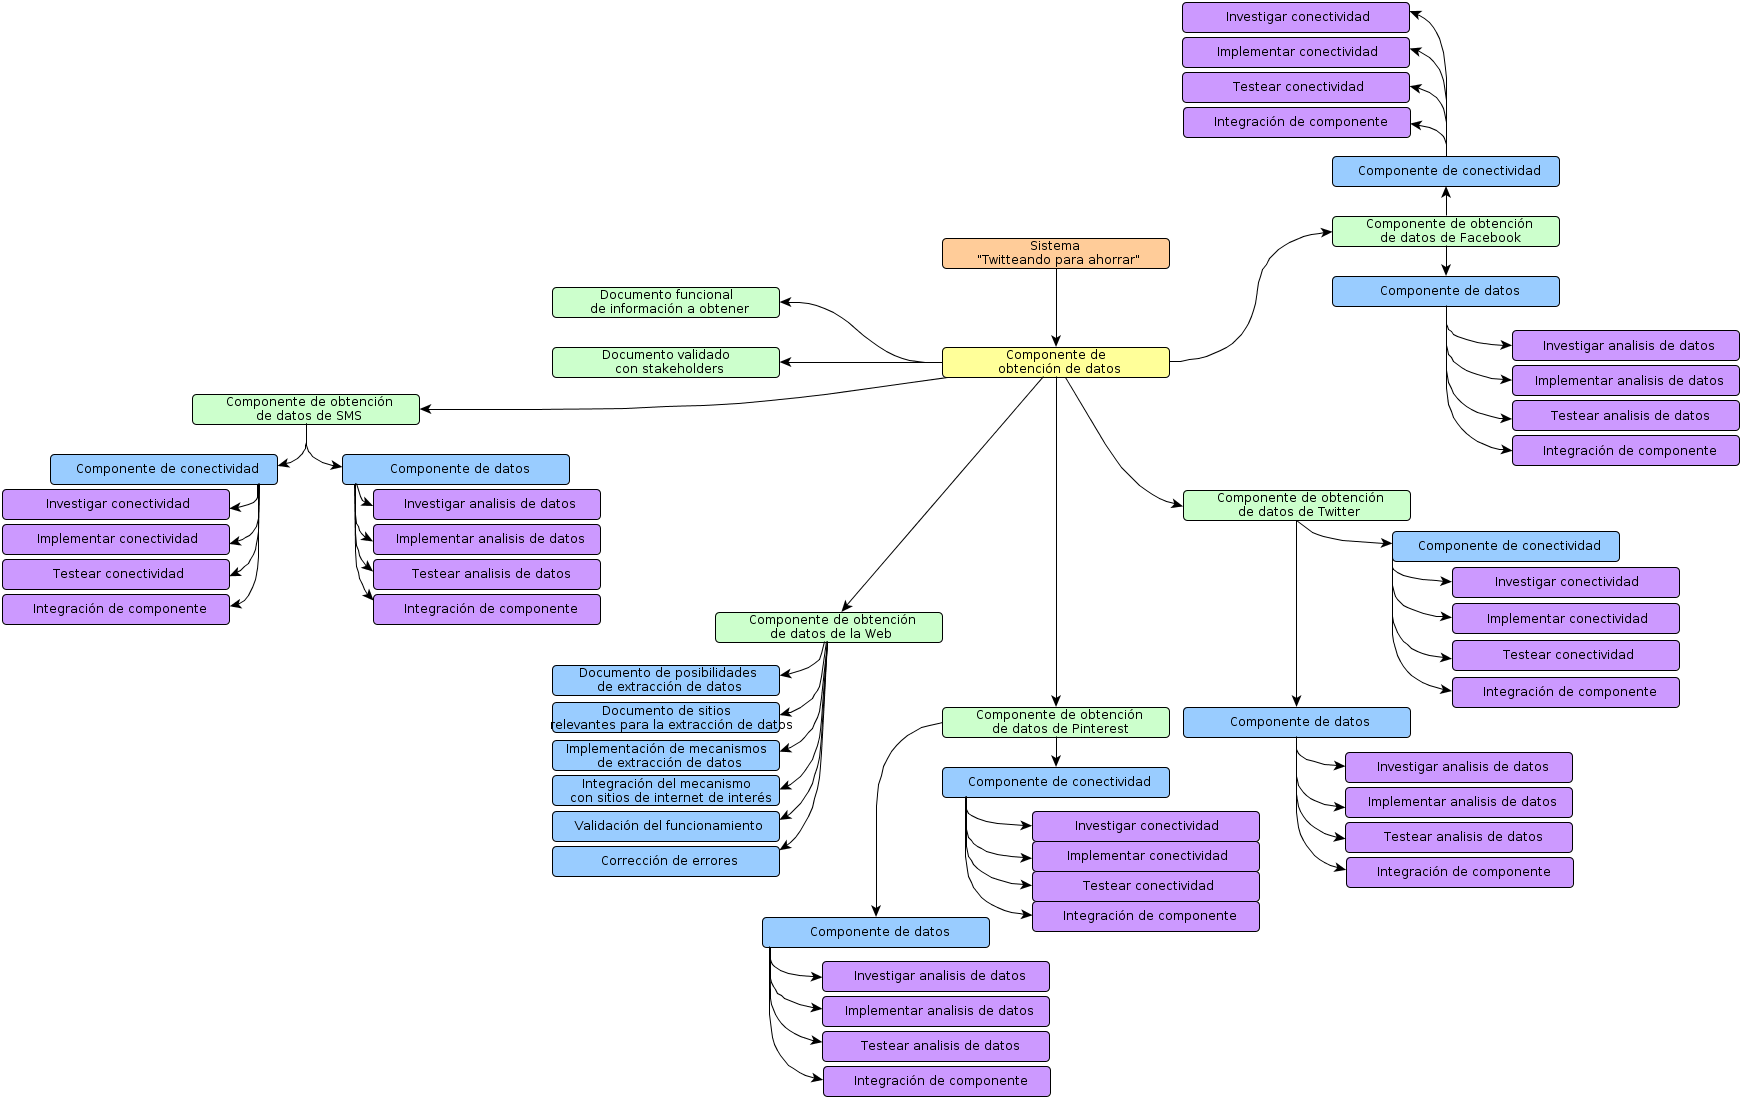
\includegraphics[scale=\escaladefault]{graficos/wbs/comp_obtencion_datos.png}
\caption{Componente de obtención de datos}
\end{figure}

\begin{figure}[H]
\centering
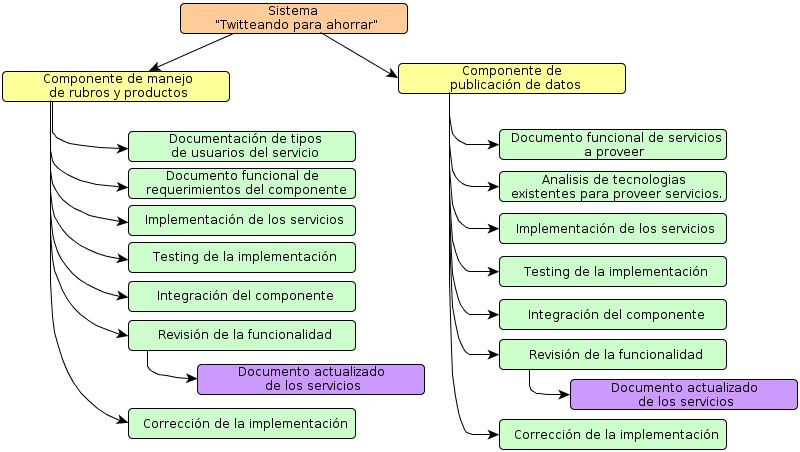
\includegraphics[scale=\escaladefault]{graficos/wbs/comp_rubros_y_api.png}
\caption{Componente de publicación de datos y componente de rubros y productos}
\end{figure}

\begin{figure}[H]
\centering
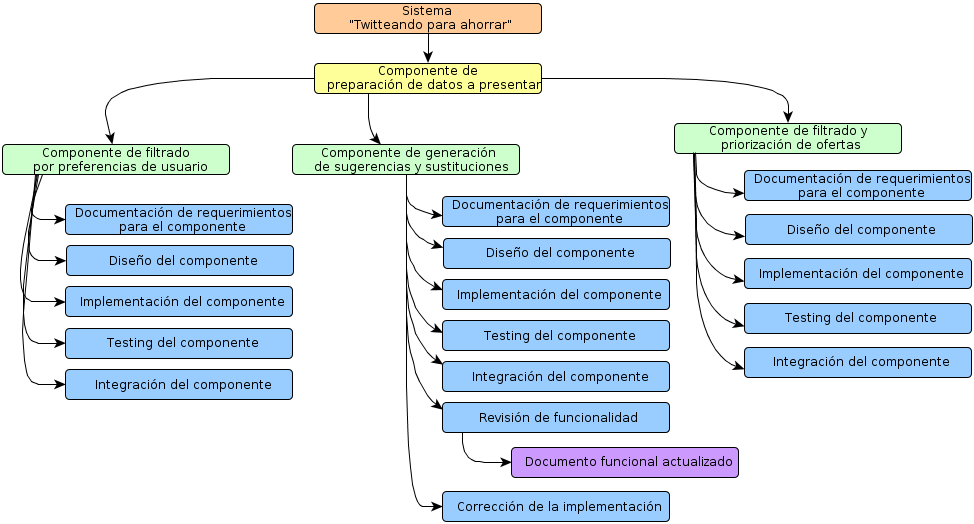
\includegraphics[scale=\escaladefault]{graficos/wbs/com_prep_de_datos.png}
\caption{Componente de preparación de datos a presentar}
\end{figure}

\begin{figure}[H]
\centering
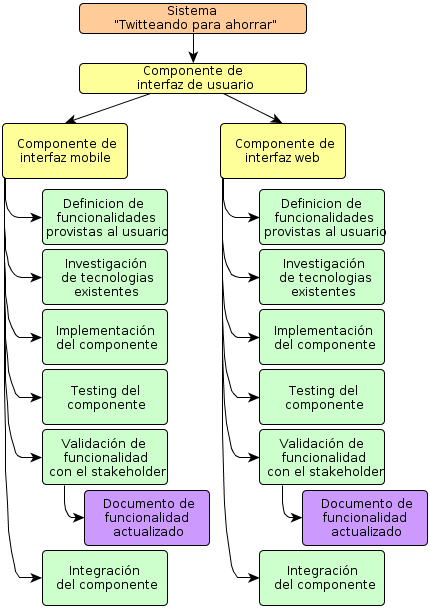
\includegraphics[scale=\escaladefault]{graficos/wbs/comp_interfaz.png}
\caption{Componente de interfaz de usuario}
\end{figure}

\begin{figure}[H]
\centering
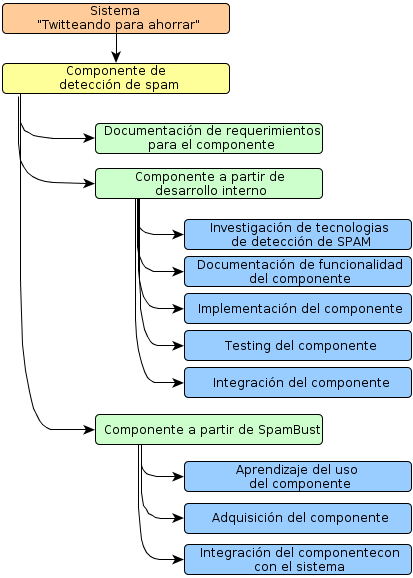
\includegraphics[scale=\escaladefault]{graficos/wbs/comp_de_spam.png}
\caption{Componente de detección de spam}
\end{figure}

\begin{figure}[H]
\centering
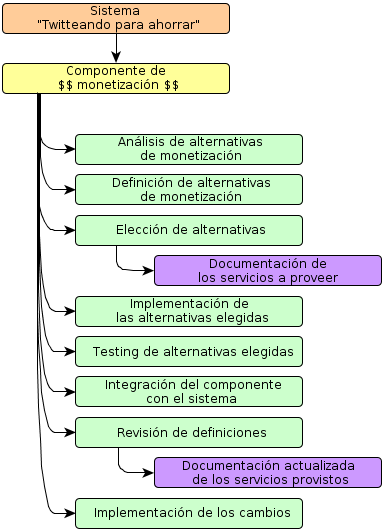
\includegraphics[scale=\escaladefault]{graficos/wbs/comp_monetizacion.png}
\caption{Componente de monetización}
\end{figure}

\begin{figure}[H]
\centering
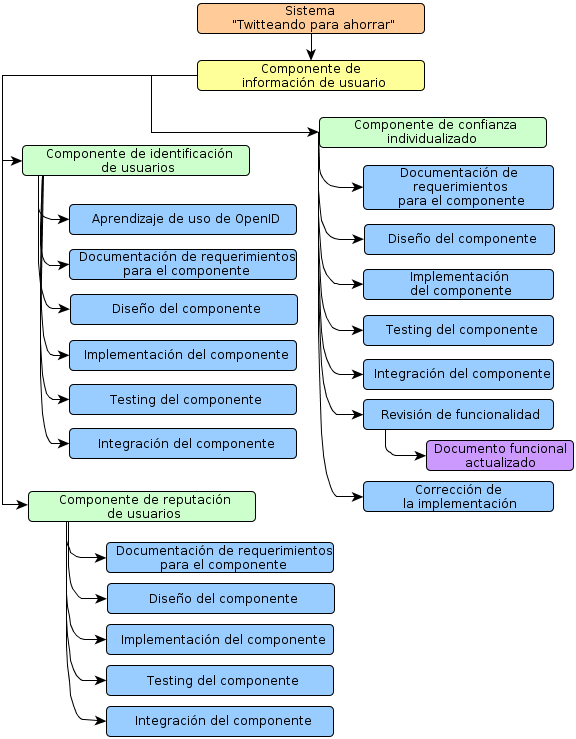
\includegraphics[scale=\escaladefault]{graficos/wbs/comp_de_info_de_usuario.png}
\caption{Componente de información de usuario}
\end{figure}

\end{document}

